\section{Simulation Validation}
\label{sec:sim}

We keep the artifact's study numbering, so the theorem-backing
simulations SS2--SS5 are reported there. The controlled checks below do
not validate unseen operational traces; they show that the computation,
analytic claims, and diagnostics behave as intended on controlled
inputs.

\subsection{SS1 and the Analytic Checks}

SS1 isolates the numerical calculation behind the reliability estimates.
We generate 500 random substochastic chains per size
$m \in \{5, 10, 50, 100, 500\}$ and compare $R_\infty$
(Proposition~\ref{thm:closed}) with Monte Carlo estimates from $10^5$
trajectories per chain, used as an independent simulation baseline for
the same fitted chain rather than as a competing estimator. The absolute
error $|R_\infty^{\rm cf} - \hat R_\infty^{\rm MC}|$ stays below the
$5\%$ acceptance threshold at every size, which supports the closed-form
computations used later in SS6 and SS9 while leaving the Markov-fit
question to the GoF protocol.

Three further controlled checks, reported in full in the artifact,
confirm the analytic claims. The perturbation bound of
Proposition~\ref{thm:perturb} tracks the true
$|R_\infty(\varepsilon)-R_\infty(0)|$ over $\varepsilon\in[0,0.28]$, so
it screens local changes by direction and scale before a full rerun. The
correlated-trial gap of Theorem~\ref{thm:corr} grows with $k$ and with
$\mathrm{Var}(p(\xi))$, confirming that agreement, pass$^k$, and the
independent-trial calculation are different projections of first-passage
behavior rather than interchangeable scalars. Finally, across six
rare-failure scaling regimes the cumulative first-passage curve
converges to the Goel--Okumoto mean-value form
(Proposition~\ref{thm:nhpp}), so Goel--Okumoto appears as a limiting case
of the agent-chain model rather than an unrelated baseline.

%% ----------------------------------------------------------------
%% [REDUCTION] SS2--SS5 (theorem-backing simulations) and the
%% figures fig_ss1_cf_vs_mc / fig_perturbation / fig_correlation_gap /
%% fig_nhpp_limit are suppressed from the 12-page body. They are
%% retained in source and in the reproducibility artifact (see
%% code/sim/SS1*--SS5*.py and figs/). The body retains SS1 as a basic
%% closed-form sanity check and SS7 (goodness-of-fit protocol
%% validation) as the statistical foundation for SS9.
%% ----------------------------------------------------------------
\iffalse
\begin{figure}[!t]
  \centering
  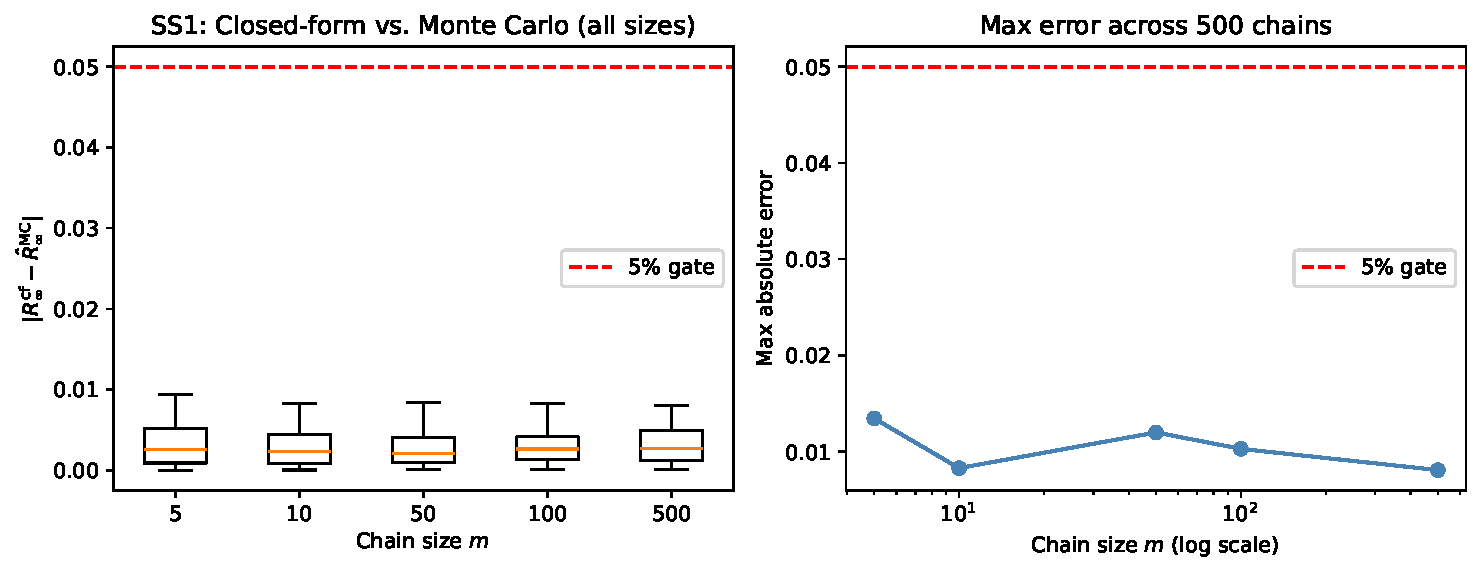
\includegraphics[width=\columnwidth]{../figs/fig_ss1_cf_vs_mc.pdf}
  \caption{SS1 closed-form validation: absolute error
           $|R_\infty^{\rm cf} - \hat{R}_\infty^{\rm MC}|$ between
           analytic eventual-success reliability and Monte Carlo
           estimates across 500 chains per size. All errors are below
           the 5\% G2 threshold.}
  \label{fig:ss1}
\end{figure}

\begin{figure}[!t]
  \centering
  \begin{minipage}[t]{0.32\columnwidth}
    \centering
    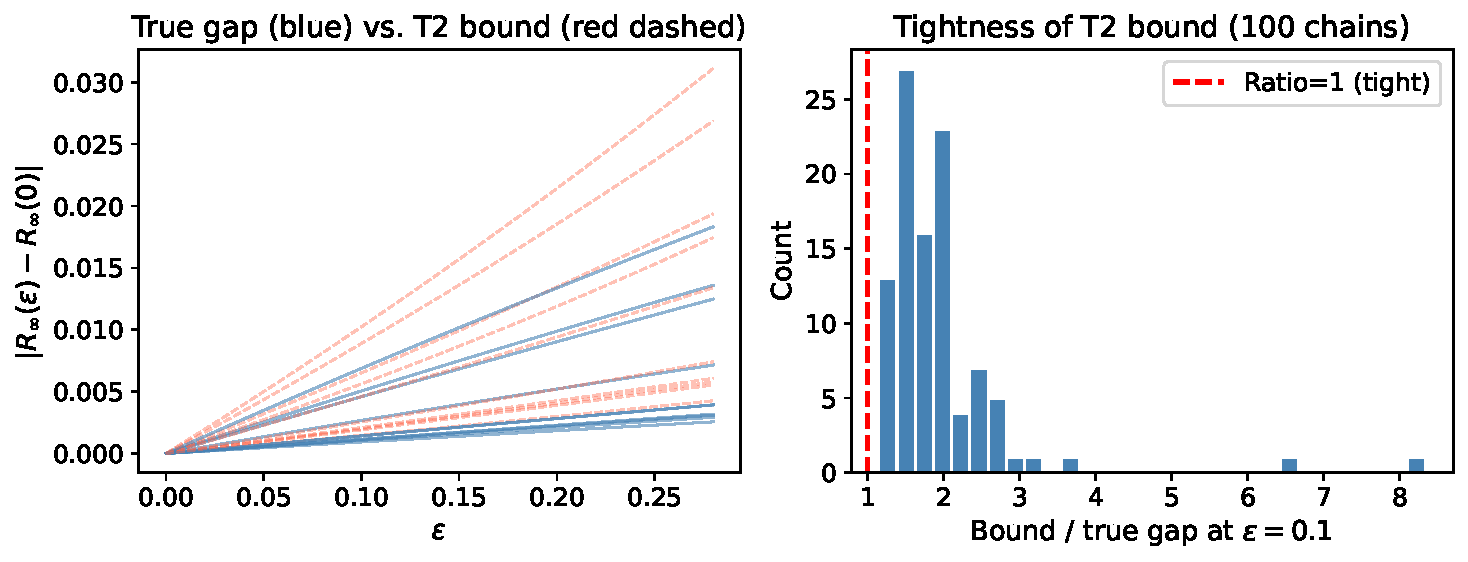
\includegraphics[trim=0bp 0bp 350bp 0bp,clip,width=\linewidth,height=0.075\textheight,keepaspectratio]{../figs/fig_perturbation.pdf}\\[-0.3ex]
    {\scriptsize (a) Perturbation}
  \end{minipage}\hfill
  \begin{minipage}[t]{0.32\columnwidth}
    \centering
    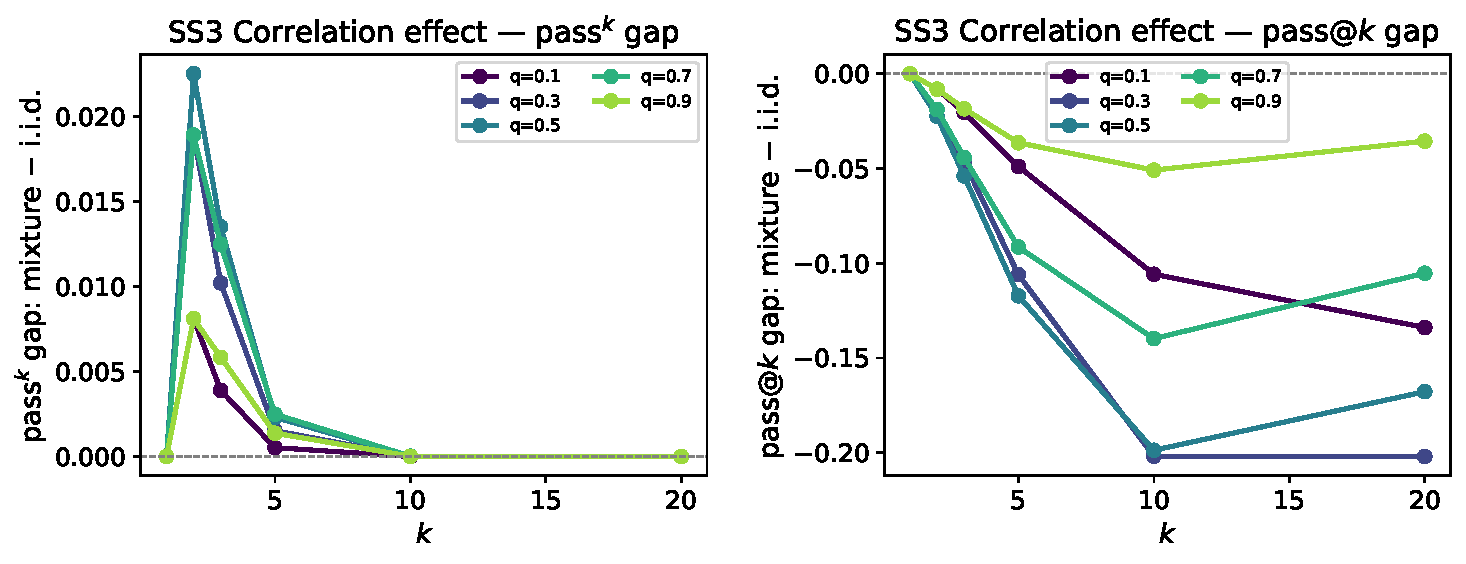
\includegraphics[trim=0bp 0bp 365bp 0bp,clip,width=\linewidth,height=0.075\textheight,keepaspectratio]{../figs/fig_correlation_gap.pdf}\\[-0.3ex]
    {\scriptsize (b) Agreement}
  \end{minipage}\hfill
  \begin{minipage}[t]{0.32\columnwidth}
    \centering
    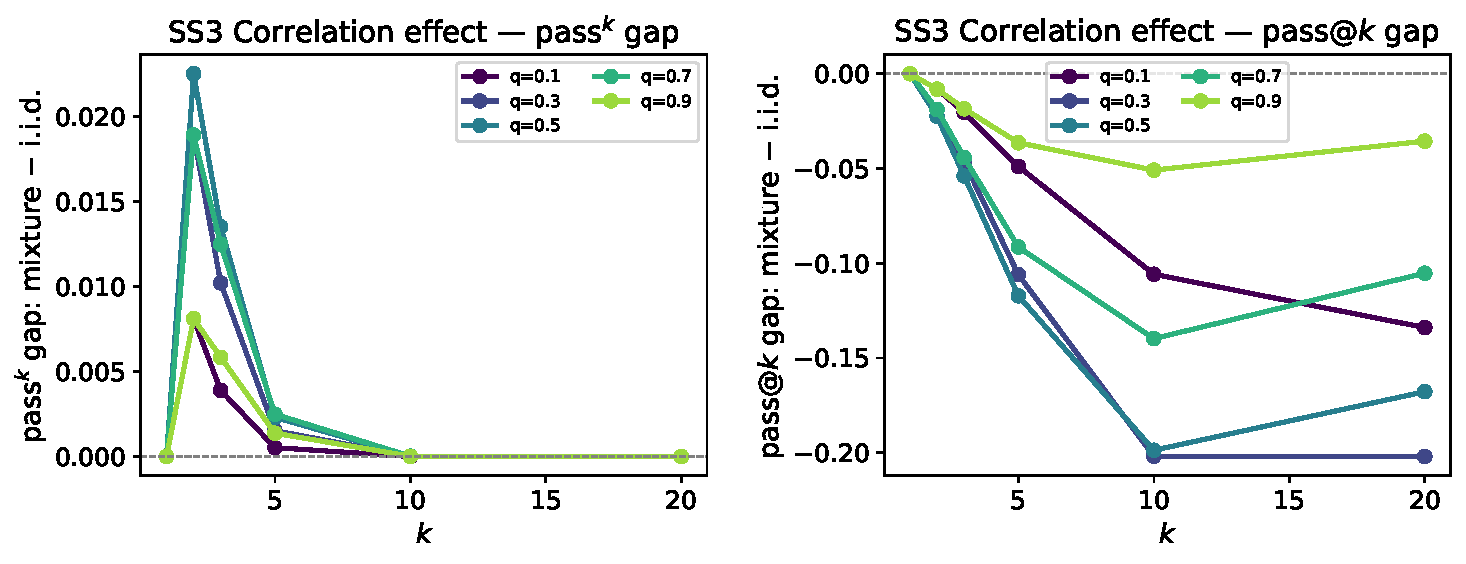
\includegraphics[trim=365bp 0bp 0bp 0bp,clip,width=\linewidth,height=0.075\textheight,keepaspectratio]{../figs/fig_correlation_gap.pdf}\\[-0.3ex]
    {\scriptsize (c) pass$^k$}
  \end{minipage}
  \caption{Additional theorem checks retained in the artifact:
           (a) perturbation bound behavior, (b) correlated-trial
           agreement lift, and (c) pass$^k$ gap.}
  \label{fig:analytic_checks}
\end{figure}

\begin{figure}[!t]
  \centering
  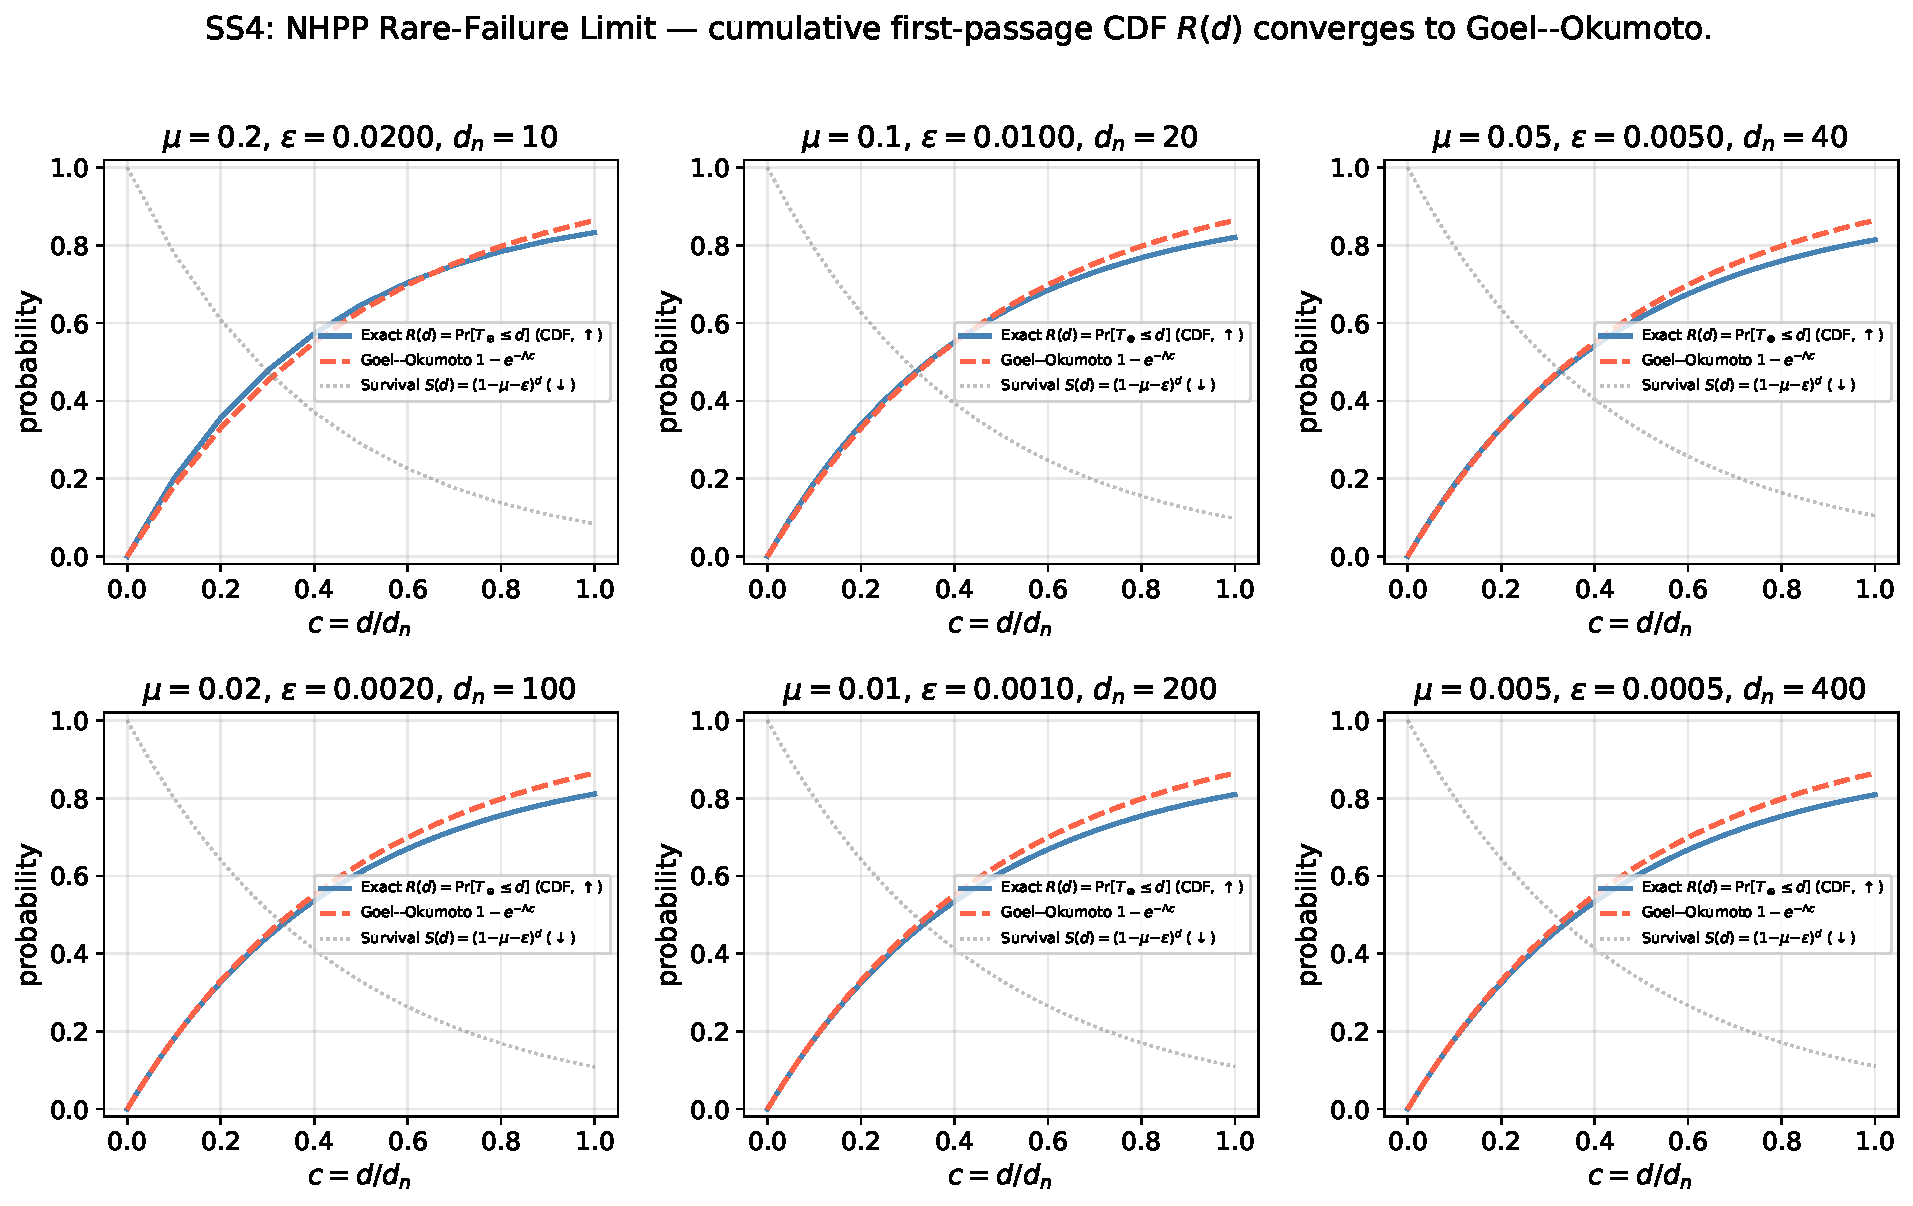
\includegraphics[width=\columnwidth,height=0.16\textheight,keepaspectratio]{../figs/fig_nhpp_limit.pdf}
  \caption{Goel--Okumoto rare-failure limit check: the cumulative
           first-passage distribution of the fitted-chain model
           approaches the NHPP mean-value form across six scaling
           regimes.}
  \label{fig:goel_okumoto_limit}
\end{figure}

\subsection{SS2: Perturbation Bound Tightness}

For 100 chains ($m=10$), we sweep $\varepsilon \in [0, 0.28]$ and compare
the T2 analytic bound against the true $|R_\infty(\varepsilon) -
R_\infty(0)|$.

\subsection{SS3: Correlation Effect on pass$^k$}

The gap $\mathrm{pass}^k_{\rm mix} - R_\infty^k$ as a function of $k$ and
mixing probability $q$ confirms the Jensen inequality in
Theorem~\ref{thm:corr}.

\subsection{SS4: NHPP Limit Verification}

We generate a sequence of 1-state agent chains with per-step success
rate $\mu_n\in\{0.2, 0.1, 0.05, 0.02, 0.01, 0.005\}$, per-step failure
rate $\varepsilon_n = 0.1\,\mu_n$, and horizon $d_n = \lceil
\Lambda/\mu_n\rceil$ with $\Lambda=2.0$. For each $n$ we compare the
\emph{cumulative first-passage CDF}
$R_n(d)=\mu_n/(\mu_n+\varepsilon_n)\cdot(1-(1-\mu_n-\varepsilon_n)^d)$
against the Goel--Okumoto mean-value function $1-e^{-\Lambda c}$ in the
rescaled horizon $c=d/d_n$. The KS distance between the two CDFs is
monotone non-increasing in $n$ and the asymptotic $p$-value exceeds
$0.05$ for all six scaling points, confirming
Proposition~\ref{thm:nhpp}. The \emph{survival} function
$S_n(d)=(1-\mu_n-\varepsilon_n)^d$ is separate from $R(d)$ and is not
what Goel--Okumoto predicts.

\subsection{SS5: PRISM Cross-Check}

We export 5 chains ($m=5$) to PRISM DTMC format and run the
query \texttt{P=? [F<=20 "success"]}.  Python closed-form matches PRISM
results to within $10^{-8}$, confirming bit-for-bit correctness.
\fi
%% [END REDUCTION — SS1/SS2/SS3/SS4/SS5 figures]

\subsection{SS7: Goodness-of-Fit of the Agent-DTMC Assumption}
\label{sec:ss7}

SS7 tests the goodness-of-fit protocol of \S\ref{sec:gof}
(Algorithm~\ref{alg:gof}) on three controlled conditions. The goal is
not to make every trace Markov, but to separate corpora where the
fitted-chain abstraction is credible from those where it is not.

\emph{(A) Markov ground truth.} On $30$ corpora of $300$ traces from a
known 1st-order absorbing chain ($m=5$), the composite test retains the
null in $100\%$ of corpora at $\alpha=0.05$; since a nominal $5\%$ test
would reject once or twice in $30$ replicates, the observed size is
\emph{conservative} rather than exactly nominal.
\emph{(B) 2nd-order ground truth.} On $15$ corpora from a 2nd-order
chain with mixture weight $0.6$, the FPT-KS layer alone rejects $0\%$
while the AIC layer rejects $100\%$ with
$\Delta_{\rm AIC}\in[+979,+1614]$, so the composite
accept-if-both-pass rule rejects $100\%$.
\emph{(C) MAST-derived self-consistency.} Sampling 500 synthetic traces
from each of the 7 MAST-derived chains of \S\ref{sec:mast}, the
composite test accepts all 7 (KS $p$-values
$\in\{0.320, 0.374, 0.541, 0.828, 0.910, 0.994, 1.000\}$, with the AIC
layer preferring the first-order model in every case). Because these
traces are sampled from the fitted chain, (C) checks internal
consistency, not whether real agent traces are Markov; the held-out
study next checks whether the full pipeline recovers first-passage
behavior on controlled MAST-style traces it did not fit.

%% [REDUCTION] fig:gof is suppressed for the 12-page body: conditions (A)--(C) above report
%% every number it plots. Retained in the artifact (figs/fig_gof.pdf).
\iffalse
\begin{figure}[!t]
  \centering
  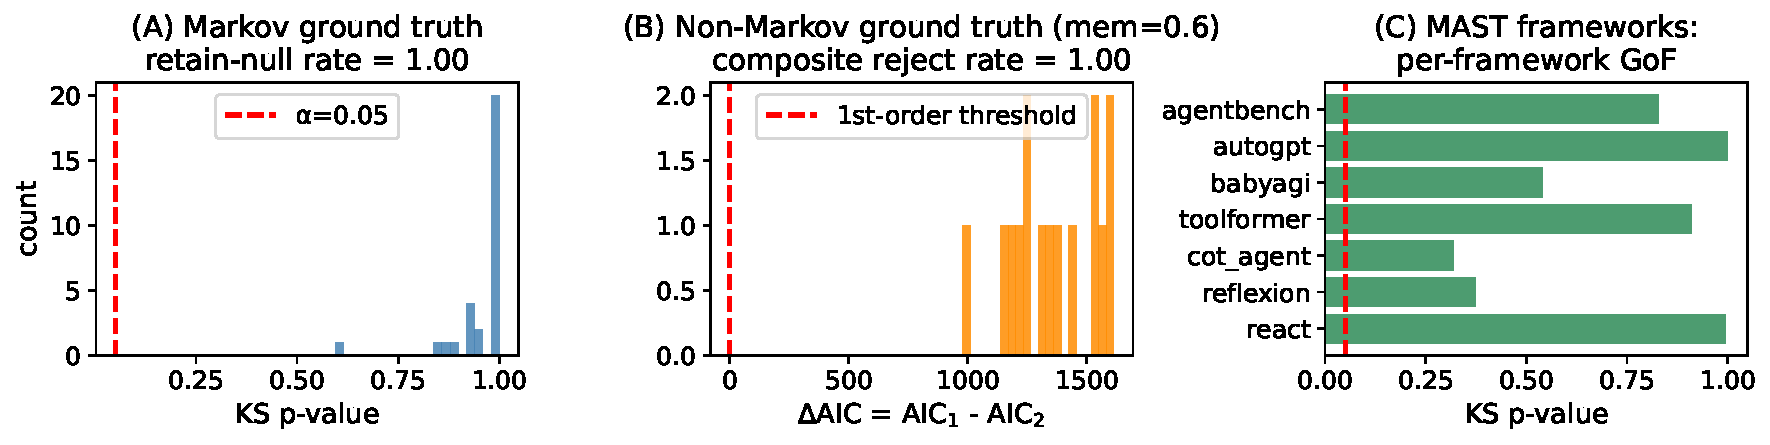
\includegraphics[width=\columnwidth]{../figs/fig_gof.pdf}
  \\[-0.3ex]
  \begin{minipage}[t]{0.32\columnwidth}
    \centering
    {\scriptsize (a) Markov ground truth: KS $p$-values}
  \end{minipage}\hfill
  \begin{minipage}[t]{0.32\columnwidth}
    \centering
    {\scriptsize (b) 2nd-order ground truth: AIC rejection}
  \end{minipage}\hfill
  \begin{minipage}[t]{0.32\columnwidth}
    \centering
    {\scriptsize (c) MAST-derived: self-consistency KS}
  \end{minipage}
  \caption{SS7 tests the GoF safeguard across Markov ground truth,
           2nd-order ground truth, and MAST-derived self-consistency
           conditions.}
  \label{fig:gof}
\end{figure}
\fi


SS1, the artifact checks of
Propositions~\ref{thm:perturb} and~\ref{thm:nhpp} and
Theorem~\ref{thm:corr}, and SS7 thus form a validation ladder that separates numerical correctness, analytic
behavior, and diagnostic behavior from the held-out recovery tested
next.

%% ================================================================
